\section{Motion Manifold Flow Primitives} 
We begin this section by introducing the notations and assumptions used throughout the paper. Let \({\cal Q}\) be a configuration space, and denote a sequence of configurations by \(x = (q_1, \ldots, q_T)\), referred to as a trajectory, where \(q_i \in {\cal Q}\) for all \(i\) and \(T\) is a fixed positive integer representing the length of trajectory. The trajectory space is then denoted by \({\cal X} = {\cal Q}^T\), which is typically very high-dimensional.
We denote the task parameter by \(c \in {\cal C}\) and assume access to a trajectory-task pair dataset \({\cal D} = \{(x^i, c^i)\}_{i=1}^{N}\), where many-to-many correspondences exist between \(x\) and \(c\) (e.g., multiple values of \(c\) may correspond to the same \(x\) and vice versa).

In the subsequent sections, we first explain the limitations of existing task-conditioned motion manifold primitives, introduce our Motion Manifold Flow Primitives (MMFP), and describe its specific application when the task parameter is a free-form text input.

\subsection{Limitations of existing motion manifold primitives}
\label{sec:limit}
Existing motion manifold-based models, TCVAE~\cite{noseworthy2020task} and MMP~\cite{lee2023equivariant}, adopt conditional autoencoder architectures for task-conditioned trajectory generation. Both assume a lower-dimensional latent space \({\cal Z}\) and train an encoder \(g : {\cal X} \to {\cal Z}\) and a conditional decoder \(f : {\cal Z} \times {\cal C} \to {\cal X}\) (or their stochastic variants) that map a trajectory \(x\) to a latent representation \(z\) and generate a trajectory given \((z, c)\). The latent prior \(p_{\rm prior}(z)\) is typically modeled as a Gaussian or a Gaussian mixture model. Motion sampling involves drawing \(z\) from the prior and mapping it through the decoder \(f\).

We note that the latent prior is {\it shared} across all task parameters, requiring the conditional decoder to sufficiently distort the same prior into different motion distributions based on the task parameter. However, when motion distributions shift dramatically (complex task-motion dependencies), the decoder often struggles to capture the complex nonlinear transformations required. In contrast, probability flow-based models continuously transform the prior via an ODE, where smooth, incremental changes accumulate into significant variations, making them better suited for modeling such complex dependencies.

\subsection{Decoupling manifold learning and conditional densities}
Our Motion Manifold Flow Primitives (MMFP) framework consists of two modules: (i) motion manifold and (ii) latent flow.
The motion manifold model consists of two neural networks, an encoder $g:{\cal X} \to {\cal Z}$ and a decoder $f:{\cal Z} \to {\cal X}$, which are trained as follows:
\begin{equation}
    \min_{f,g} \frac{1}{N}\sum_{i=1}^{N} d^2(x^i, f(g(x^i))) + \eta \| g(x^i)\|^2 + \delta {\cal E}(f,g),
\end{equation}
where $\eta,\delta$ are some positive scalars. The second term penalizes the norm of latent values to prevent them from diverging excessively far from the origin. The third term is added to ensure their smoothness, which is defined as follows: ${\cal E}(f,g):= \mathbb{E}_{z} \big[ \sum_{t=1}^{T-1} \| f^{t+1}(z) - f^t(z)\|^2 \big]$, where $f(z) = (f^1(z), \ldots, f^T(z)) \in {\cal Q}^T$.
The latent value \( z \) in this expectation is sampled with augmentation as \( z = \alpha g(x^i) + (1-\alpha) g(x^j) \), where \( \alpha \sim {\cal U}[-0.4, 1.4] \) and \( x^i, x^j \) are sampled from the dataset, to extend the regularization effect to regions where data is not available, adopting~\cite{yonghyeon2022regularized}.

Given a pre-trained encoder \(g\), generate a set of latent-task pairs \(\{(z^i, c^i)\}_{i=1}^N\) where \(z^i = g(x^i)\). A neural network vector field \(v_s(z, c)\) is then trained using the flow matching loss in (\ref{eq:cfmloss}). Finally, given a task parameter \(c\), motion sampling is performed by integrating the ODE \(dz/ds = v_s(z, c)\) from \(s=0\) to \(s=1\) to obtain latent samples \(z_1\) (where the index denotes the final time step \(s=1\)), followed by decoding them using \(f : z_1 \mapsto x\).


A reasonable question may arise: Why not use diffusion models~\cite{song2020score}, which are modeled with stochastic differential equations (SDEs), instead of flow matching models based on ordinary differential equations (ODEs), in the latent space? One answer is that while both approaches can capture complex conditional dependencies, flow matching models enable faster generation~\cite{lipman2022flow}.
Moreover, given a limited dataset size, flow matching tends to achieve better interpolation and generalization compared to diffusion models, as optimal transport paths used in flow matching are smoother than the diffusion paths~\cite{lipman2022flow}. Our empirical studies further support this, showing that latent flow models outperform latent diffusion models; see Section~\ref{sec:toy_exp}.

\subsection{Language as a task parameter}
\begin{figure*}
    \centering
    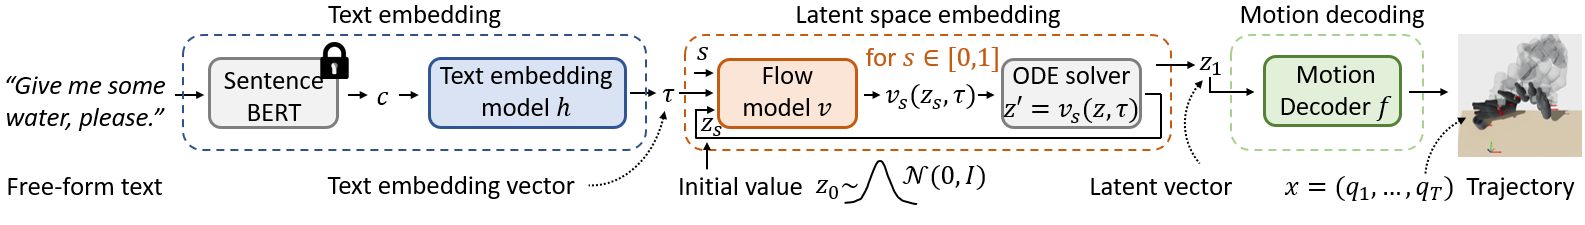
\includegraphics[width=\linewidth]{tabs/figures/ral_mmfp_language.png}
    \caption{The procedure of motion generation in MMFP: (i) the Sentence-BERT encodes a free-form text into a vector $c$, (ii) the text embedding model $h$ maps $c$ to a text embedding vector $\tau$, (iii) we solve the ODE $z'=v_s(z,\tau)$ from $s=0$ to $s=1$ with an initial value $z_0$ sampled from Gaussian ${\cal N}(z|0,I)$ and obtain $z_1 \in {\cal Z}$, and (iv) the motion decoder $f$ maps $z_1$ to a trajectory $x=(q_1,\ldots,q_T)$.}
    \label{fig:method}
\end{figure*}

We use a pre-trained text encoder, Sentence-BERT~\cite{reimers-2019-sentence-bert}, without fine-tuning, to encode free-form texts into 768-dimensional vectors. These vectors serve as task parameters, denoted by \(c\). However, we empirically observed that directly inputting the 768-dimensional task parameter into the velocity model \(v_s(z,c)\) does not produce satisfactory results. To address this limitation, we introduce a text embedding model, a neural network \(h\), which encodes \(c\) into a lower-dimensional vector \(\tau \in \mathcal{T}\).

We train the text embedding model $h: c \mapsto \tau$ and velocity field $v: (s,z,\tau) \mapsto dz/ds$ simultaneously with the following {\it regularized} flow matching loss:

{\small
\begin{equation}
   \label{eq:lfl}
   \sum_{i,k} \mathbb{E}_{s,z_0} \big[\|v_s(z_s^i, h(c^i)) - (z^i - z_0)\|^2\big] + \gamma \|h(c^i) - h(\tilde{c}^{ik})\|^2 ,
\end{equation}
}
where $z_s^i = (1-s)z_0 + s z^i$, and $s, z_0$ are sampled from $\mathcal{U}[0,1]$ and a Gaussian prior, respectively. The second term, scaled by a positive weight \(\gamma\), encourages robustness against diverse text variations. Here, \(\tilde{c}^{ik}\) for $k=1,\ldots,K$ are Sentence-BERT encoding vectors with meanings similar to those of \(c^i\), generated using the Large Language Model \textit{ChatGPT}. 
We refer to Fig.~\ref{fig:method} for an overview of the motion sampling procedure using MMFP given a free-form text input.
